\documentclass[10pt]{beamer}

%% Use this for 4 on 1 handouts
%\documentclass[handout]{beamer}
%\usepackage{pgfpages}
%\pgfpagesuselayout{4 on 1}[landscape, a4paper, border shrink=5mm]

\usepackage[english]{babel}
\usepackage[utf8]{inputenc}
\usepackage[T1]{fontenc}
\def\subitem{\item[\hspace{1.5cm} -]}


% Set the presentation mode to BTH
\mode<presentation>
{
	\usetheme{BTH_msv}
	% Comment this if you do not want to reveal the bullets before they are going to be used
	\setbeamercovered{transparent}
}


% Information for the title page

\title[]{Introduction to Project}
\subtitle{Cloud Computing}
%\date[]{}

\author[Mikael Svahnberg]{Mikael Svahnberg\inst{1}}
\institute[BTH] % (optional, but mostly needed)
{
  \inst{1}%
 Mikael.Svahnberg@bth.se\\
 School of Computing\\
 Blekinge Institute of Technology%
}

% Delete this, if you do not want the table of contents to pop up at
% the beginning of each subsection:
%\AtBeginSubsection[]
%{
%  \begin{frame}<beamer>{Outline}
%    \tableofcontents[currentsection,currentsubsection]
%  \end{frame}
%}


% If you wish to uncover everything in a step-wise fashion, uncomment
% the following command: 
%\beamerdefaultoverlayspecification{<+->}

\begin{document}

% Titlepage frame
\begin{frame}
  \titlepage
\end{frame}

% ToC frame
% Use \section and \subsection commands to get things into the ToC.
%\begin{frame}
 %\frametitle{Outline}
 % \tableofcontents
%\end{frame}

% -----------------------------
% Your frames goes here
% -----------------------------

\begin{frame}[t]
\frametitle{Goals of the Project}

From Course Syllabus:
\vspace{0.5cm}

\begin{scriptsize}
Kunskap och Förståelse:
\begin{itemize}
\item Kunna ingående förklara de grundläggande teknologier som används i cloud-system
\item Kunna ingående resonera om privacy och security i cloud-system
\end{itemize}

Färdighet och förmåga
\begin{itemize}
\item Kunna designa och implementera en cloud-applikation
\item Kunna driftsätta, testa, och övervaka en cloud-applikation
\item Kunna optimera en cloud-applikation med avseende på relevanta kvalitetsegenskaper
\item Kunna använda sig av en existerande hypervisor
\item Kunna starta virtuella maskiner på en existerande hypervisor
\item Kunna genomföra enkel lastbalansering på en existerande hypervisor som körs på ett serverkluster
\end{itemize}

Värderingsförmåga och förhållningssätt

\begin{itemize} 
\item Kunna resonera om energianvändningen för en cloud-applikation
\item Kunna resonera om den långsiktiga evolutionen av en cloud-applikation
\end{itemize}
\end{scriptsize}
\end{frame}

\begin{frame}[t]
\frametitle{Overview}
\begin{itemize}[<+->]
\item Select and briefly describe a Project
\item Create a business case\\
  (with particular focus on why it is a good idea to use cloud resources)
\item Develop a software architecture
\item Develop a plan for your different deplopyment environments
\item Setup provisioning for your application
\item {\color{green} [Checkpoint]} Present your architecture and your deployment plan
\item Develop a test plan\\
  (that at least partially enables automated tests)
\item Implement your project
\item {\color{green} [Checkpoint]} Deploy your project
\item {\color{green} [Checkpoint]} Write an experience report
\end{itemize}
\end{frame}

\begin{frame}[t]
\frametitle{The general idea}
\begin{itemize}
\item In lab 1 you learn the basic mechnanics
\item Many challenges will not be visible in a dry lab exercise
\item With this project you encounter at least a subset of ``real-life'' challenges.
\end{itemize}

\centering
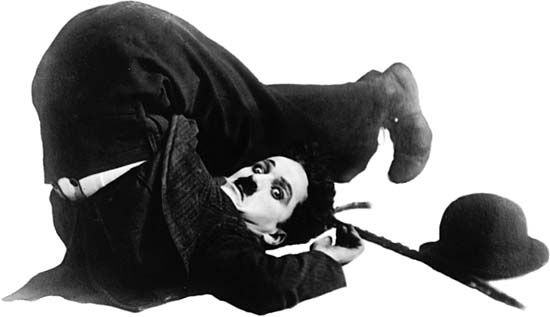
\includegraphics[height=4cm]{Chaplin_Fall.jpg}

\end{frame}

\begin{frame}[t]
\frametitle{The general idea}

\begin{columns}
\begin{column}{9cm}
\begin{itemize}
\item This should be fun!
\item Therefore, you pick your own project
\item We may advice you to complicate matters\\
  -- so you also learn what you are expected to.
\item Reflections: Take conscious decisions, summarise in a report.
\item Keep in mind the ``Cloud Investigation'' assignment.
\end{itemize}
\end{column}
\begin{column}{3cm}
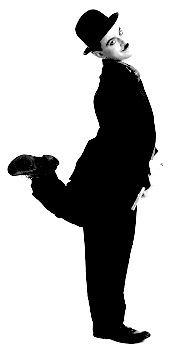
\includegraphics[height=6cm]{Chaplin_Fakeit.jpg}
\end{column}
\end{columns}
\end{frame}


% -----------------------------


%% All of the following is optional and typically not needed. 
%\appendix
%\begin{frame}[allowframebreaks]
%  \frametitle{For Further Reading}
%    
%  \begin{thebibliography}{10}
%    
%  \beamertemplatebookbibitems
%  % Start with overview books.

%  \bibitem{Author1990}
%    A.~Author.
%    \newblock {\em Handbook of Everything}.
%    \newblock Some Press, 1990.
%     
%  \beamertemplatearticlebibitems
%  % Followed by interesting articles. Keep the list short. 

%  \bibitem{Someone2000}
%    S.~Someone.
%    \newblock On this and that.
%    \newblock {\em Journal of This and That}, 2(1):50--100,
%    2000.
%  \end{thebibliography}
%\end{frame}

\end{document}


